%%%%%%% By Michał Swoboda
%%%%%%% Poprawki by Błażej Kowalczyk
%%%%%%% Uporządkował pewne rzeczy Bartłomiej Kurosz

\documentclass[xcolor=dvipsnames]{beamer}%[hyperref={pdfpagelabels=false}]{beamer}
\usepackage{lmodern}
\usepackage{polski}
\usepackage[utf8]{inputenc}
\usepackage{amsfonts}
\usepackage{tikz}

%%%%%%%%%%%%%%%% Początek poleceń własnych
% Maksymalna dostępna wysokość pola w~prezentacji (między wąskim nagłówkiem a~stopką)
% dobrana eksperymentalnie - może w~przyszłości po prostu ją wyliczać???
\newlength{\maxheight}
\setlength{\maxheight}{\paperheight}
\addtolength{\maxheight}{-17.85pt}  % tyle zajmuje naczółek ze stopką 

% Polecenie do dokładania wycentrowanych rzeczy (zdjęć) na środku slajdu 
% bez tytulariów (ale ze stopką i~naczółkiem)
% By uzyskać obrazek "na całą stronę" jako argumentu należy użyć
% 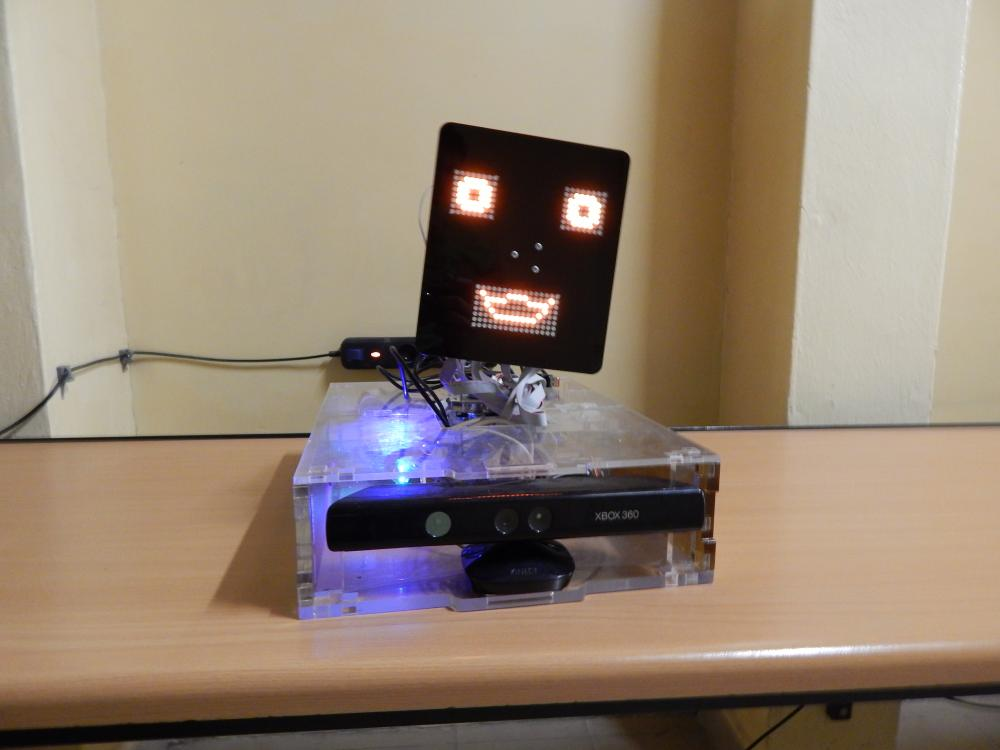
\includegraphics[height=\maxheight,width=\paperwidth]{figure/balbina.jpg}
% Jeśli nie chcesz zmian proporcji - zrezygnuj z~jednego z~wymiarów
% Obrazki za duże przykryją naczółek strony
% By wszystko było na swoim miejscu potrzebna jest dwukrotna kompilacja 
\newcommand{\framecentered}[1]{
  \setbeamertemplate{background canvas}{}
  \begin{frame}[c]
    \begin{tikzpicture}[overlay, remember picture]
      \node[anchor=center] at (current page.center) 
      {#1};
    \end{tikzpicture}
  \end{frame}}
%%%%%%%%%%%%%%%% Koniec poleceń własnych

%%%%%%%%%%%%%%%%Początek ustawień
\usebackgroundtemplate{%
  
\includegraphics[width=\paperwidth,height=\paperheight]{background/tlo.pdf}} 

\usepackage{beamerthemesplit}
\useoutertheme{infolines}
\useinnertheme{rounded}

\definecolor{konar2}{RGB}{240,152,52}
\definecolor{konar}{RGB}{151,58,66}

\setbeamercolor{block title}{fg=black,bg=konar2}
\setbeamercolor{block title alerted}{fg=konar2,bg=black}

\setbeamertemplate{navigation symbols}{}
\setbeamercolor{frametitle}{fg=white,bg=konar}
\setbeamercolor{section in head/foot}{bg=konar}
\setbeamercolor{author in head/foot}{fg=Black,bg=konar2}
\setbeamercolor{date in head/foot}{fg=Black}
\setbeamercolor{title in head/foot}{fg=white, bg=konar}
\setbeamercolor{section in head/foot}{fg=white}
\setbeamercolor{titlelike}{fg=black}
\setbeamercolor{structure}{bg=black, fg=konar2}
\setbeamercolor{subsection in head/foot}{fg=black}
\setbeamercolor{item}{bg=white}

%%%%%%%%%%%%%%%%%Koniec Ustawień

%%%%%%%%%%%%%%%%% SLAJD TYTUŁOWY

\title{Rewizja kodu}
\subtitle{Nieoczywista sztuka konstruktywnej krytyki}
\author{Jacek Jankowski}
\date{\today}  %data

%%%%%%%%%%%%%%%%%



\begin{document}

\begin{frame}
	\titlepage
\end{frame}

\begin{frame}
	\frametitle{Szybka ankieta}
	\begin{center}
		\begin{itemize}
			\item Nigdy nie miałem rewizji.
			\item Rewizje są obowiązkową częścią procesu.
			\item Więcej sprawdzam niż sam piszę.
		\end{itemize}
	\end{center}
\end{frame}

\begin{frame}
	\frametitle{Charakter pracy - oczekiwania}
	\begin{center}
		\begin{minipage}{0.45\textwidth}
			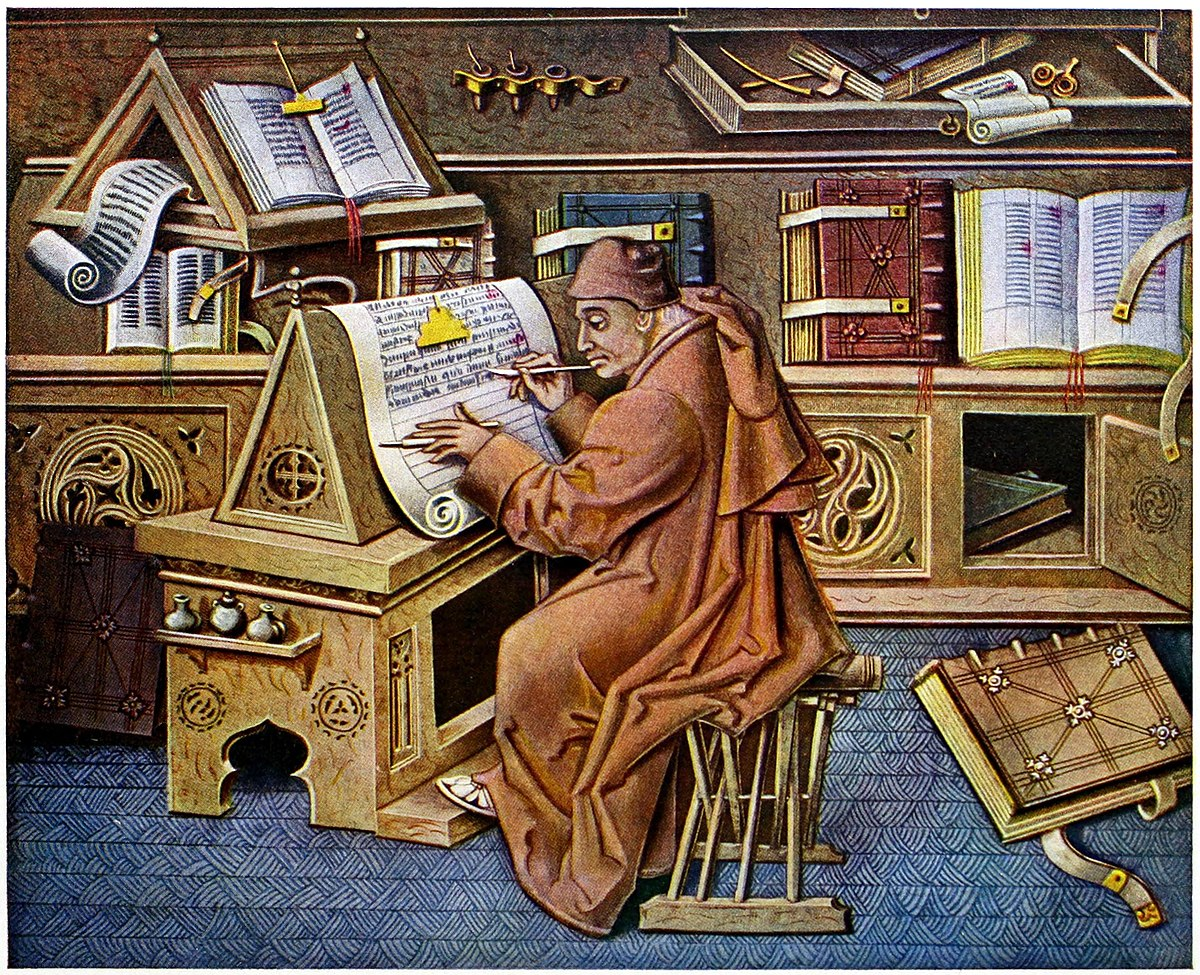
\includegraphics[width=\textwidth]{figure/skryba.jpg}
		\end{minipage}
		\begin{minipage}{0.45\textwidth}
			
\includegraphics[width=\textwidth]{figure/programista.jpg}
		\end{minipage}
	\end{center}
	\note{W poszwechnym odczuciu programista jest współczesnym odpowiednikiem skryby.}
	\note{Pracuje sam, w wielkim skupieniu, od początku do końca.}
	\note{Stanowisko idealne dla introwertyków, autystyków, nerdów etc.}
\end{frame}

\begin{frame}
	\frametitle{Charakter pracy - rzeczywistość}
	\begin{center}
		\begin{minipage}{0.45\textwidth}
			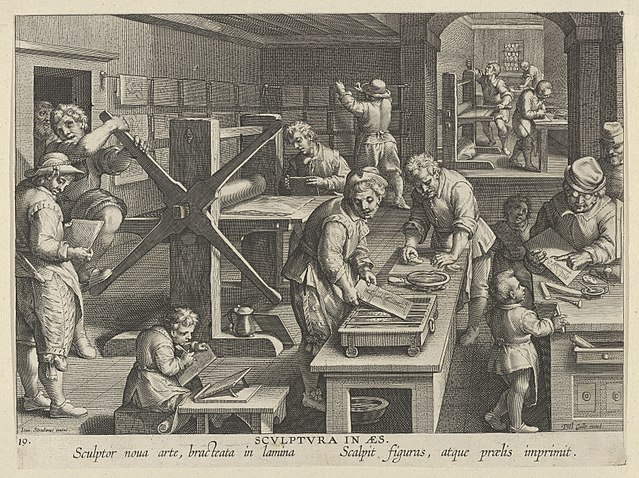
\includegraphics[width=\textwidth]{figure/drukarnia.jpg}
		\end{minipage}
		\begin{minipage}{0.45\textwidth}
			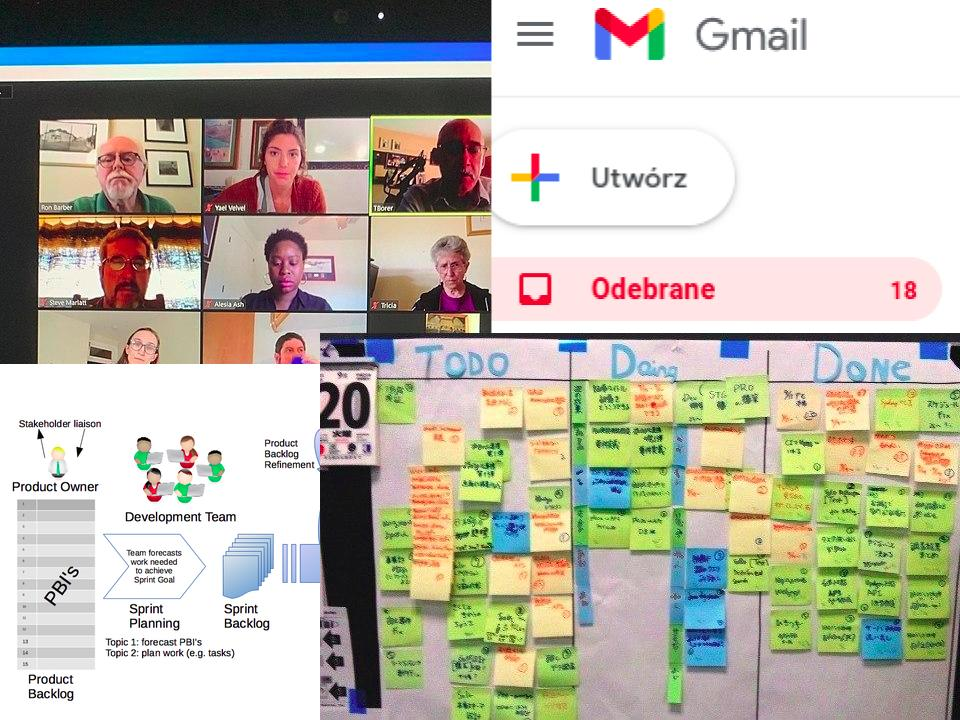
\includegraphics[width=\textwidth]{figure/disappointment.jpg}
		\end{minipage}
	\end{center}
	\note{Podstawowym problemem była czasochłonność.}
	\note{Drukarnie i dobrze zorganizowane zespoły są szybsze niż jeden człowiek :(}
	\note{Jeden programista nie jest w stanie zrobić wszystkiego!}
	\note{Za dużu funkcjonalności do zakodowania.}
	\note{Jack of all trades, master of none.}
\end{frame}

\framecentered{
	
\includegraphics[width=\textwidth,height=\textheight,keepaspectratio]{figure/no_time.jpg}
	\note{Po co? Przecież to strata czasu i nerwów.}
	\note{Dodatkowe źródło konfliktów.}
}

\begin{frame}
	\frametitle{Wypłaszczanie krzywej Boehm'a}
	\begin{center}
		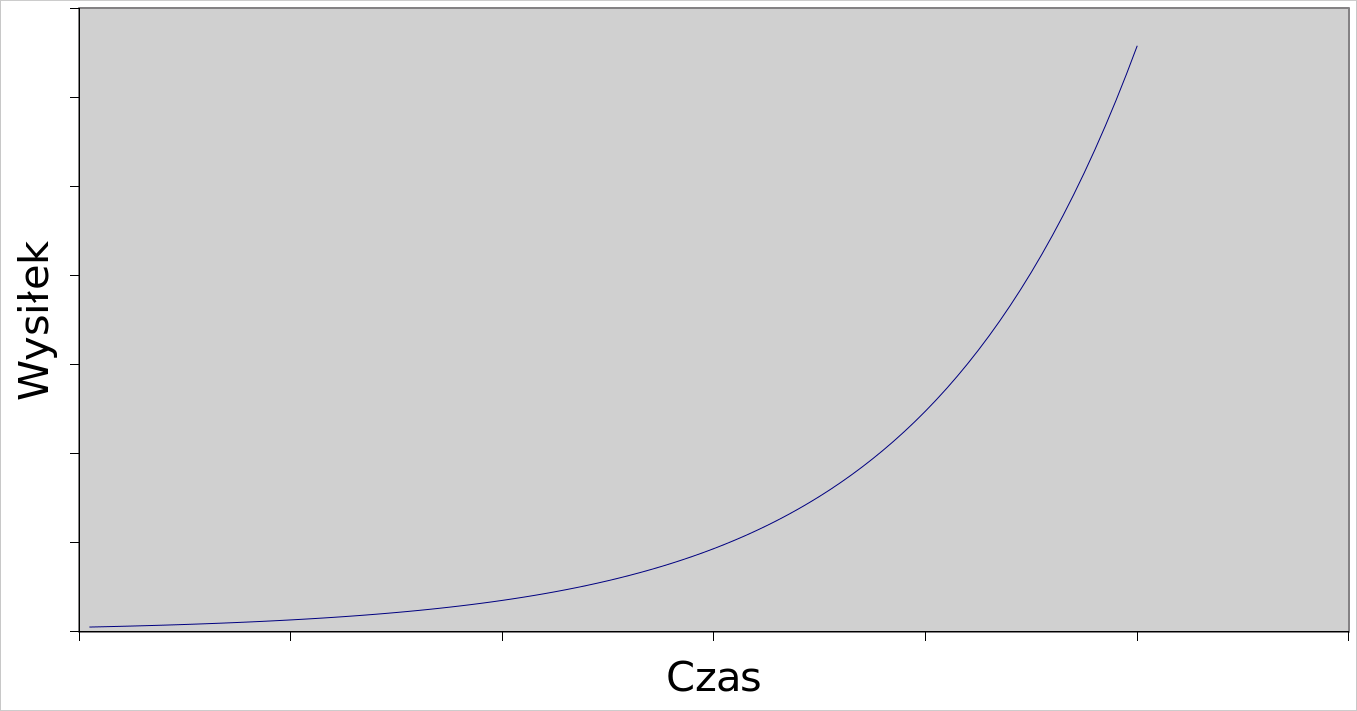
\includegraphics[width=\textwidth,height=\textheight,keepaspectratio]{figure/boehm_curve.png}
	\end{center}
\end{frame}

\begin{frame}
	\frametitle{Przyczyny akumulacji długu}
	\begin{columns}
		\begin{column}{0.5\textwidth}
			\begin{itemize}
				\item Zafiskowanie
				\item Przeoczenie
				\item Pośpiech
				\item Niewiedza
				\item Syndrom Madki
				\item Czasami po prostu się nie chce...
				\item Patologiczny przerost źródeł
				      \begin{itemize}
					      \item Zbędne wodotryski
					      \item Martwy kod
					      \item Duplikacja
				      \end{itemize}
			\end{itemize}
		\end{column}
		\begin{column}{0.5\textwidth}
			
\includegraphics[width=\textwidth,height=\textheight,keepaspectratio]{figure/dlug_techniczny.jpg}
		\end{column}
	\end{columns}
\end{frame}

\begin{frame}
	\frametitle{Jak zacząć?}
	\begin{columns}
		\begin{column}{0.5\textwidth}
			\begin{itemize}
				\item System kontroli wersji
				      \begin{itemize}
					      \item Git
				      \end{itemize}
				\item Konsensus pośród programistów
				\item Platforma do recenzowania
				      \begin{itemize}
					      \item Gerrit, GitHub, Bitbucket
				      \end{itemize}
				\item Ochrona głównej gałęzi
				      \begin{itemize}
					      \item Aplikowanie zmian tylko po review
					      \item Nikt nie może zmieniać zasad
					      \item ... z wyjątkiem DevOps'a, któremu nie zależy na terminach
				      \end{itemize}
			\end{itemize}
		\end{column}
		\begin{column}{0.5\textwidth}
			\begin{center}
				
\includegraphics[width=0.5\textwidth,keepaspectratio]{figure/podstawy.png}
			\end{center}
		\end{column}
	\end{columns}
\end{frame}

\begin{frame}
	\frametitle{Jak rozwiązać spór?}
	\begin{columns}
		\begin{column}{0.5\textwidth}
			\begin{center}
				
\includegraphics[width=\textwidth,height=0.8\textheight,keepaspectratio]{figure/rozwiazywanie_sporu.png}
			\end{center}
		\end{column}
		\begin{column}{0.5\textwidth}
			\begin{center}
				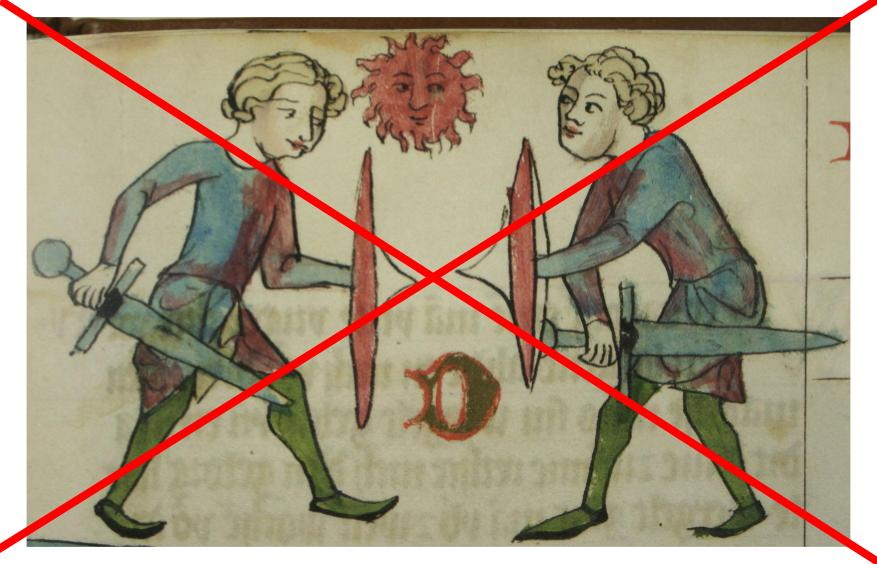
\includegraphics[width=\textwidth,height=0.8\textheight,keepaspectratio]{figure/sad_bozy.jpg}
			\end{center}
		\end{column}
	\end{columns}
\end{frame}

\begin{frame}
	\frametitle{Jak przyjąć krytykę?}
	\begin{columns}
		\begin{column}{0.5\textwidth}
			\begin{itemize}
				\item Pamiętaj, że chcą pomóc
				\item Popraw błędy i dodaj komentarze
				\item Odpowiadaj na pytania i uwagi
				\item Nie pisz w złości
				\item Rozbij za duże zmiany
			\end{itemize}
		\end{column}
		\begin{column}{0.5\textwidth}
			
\includegraphics[width=\textwidth,height=0.8\textheight,keepaspectratio]{figure/nic_osobistego.jpg}
		\end{column}
	\end{columns}
\end{frame}

\section{Koniec}
\begin{frame}
	\frametitle{Przepiękna i zjawiskowa}
	\centering \begin{figure}
		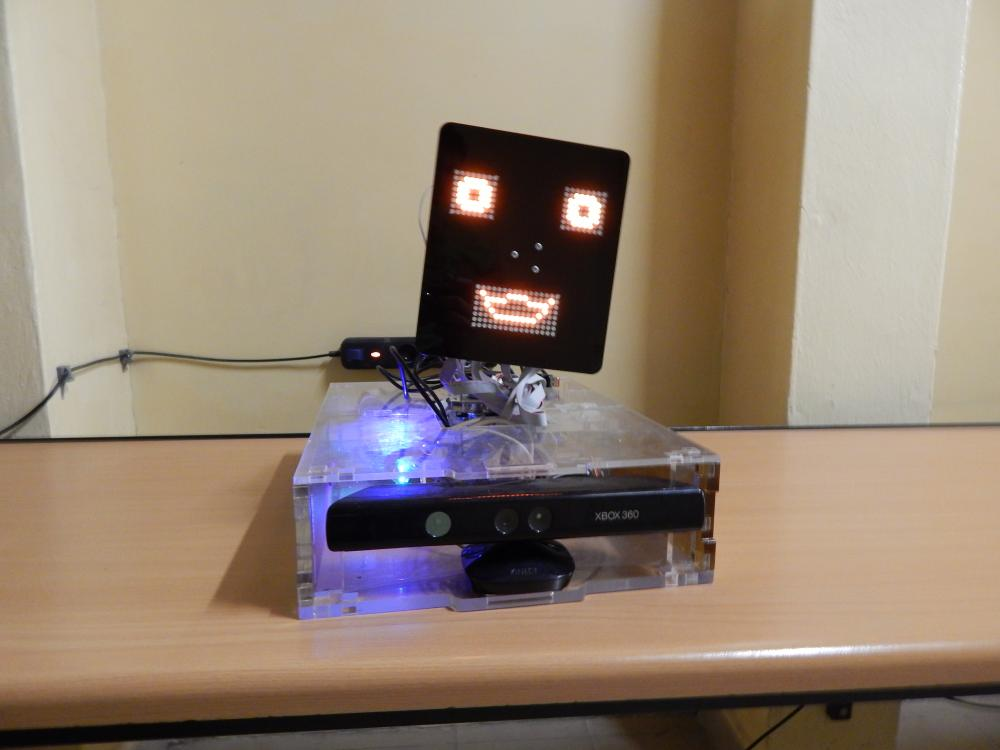
\includegraphics[height=5cm]{figure/balbina.jpg}
		\caption{Balbina}
	\end{figure}
\end{frame}

\end{document}
